\documentclass[runningheads,a4paper]{llncs}

\usepackage{amssymb}
\setcounter{tocdepth}{3}
\usepackage{graphicx}
\usepackage{tikz}
\usepackage[T1]{fontenc}
\usepackage[scaled]{beramono}
\usepackage{listings}
\usepackage{color}
\usetikzlibrary{arrows,chains,positioning,scopes,quotes,calc}
\usepackage{float}

\newcommand{\keywords}[1]{\par\addvspace\baselineskip
\noindent\keywordname\endspace\ignorespaces#1}
\pagestyle{plain}
\setlength\parindent{0pt}

\definecolor{mygreen}{RGB}{28,172,0} % color values Red, Green, Blue
\definecolor{mylilas}{RGB}{170,55,241}

\newcommand*{\StrikeThruDistance}{0.15cm}%
\newcommand*{\StrikeThru}{\StrikeThruDistance,\StrikeThruDistance}%

\tikzset{strike thru arrow/.style={
    decoration={markings, mark=at position 0.5 with {
        \draw [blue, thick,-] 
            ++ (-\StrikeThruDistance,-\StrikeThruDistance) 
            -- ( \StrikeThruDistance, \StrikeThruDistance);}
    },
    postaction={decorate},
}}

\lstset{
  language=Python,
  showstringspaces=false,
  formfeed=\newpage,
  tabsize=4,
  commentstyle=\itshape,
  basicstyle=\ttfamily,
  morekeywords={models, lambda, forms}
}

\begin{document}
\def \SystemName {Worlds} % Lol because this shit probably will change.

\mainmatter  % start of an individual contribution

% This needs some work, big time.
\title{\SystemName: A distributed MMO \textit{(DRAFT)}}

\author{Ryan Walker\\
				ryan.cjw@gmail.com}

\institute{} %Merp

\maketitle
%% Scrum area
%% TODO:
% - EXP ?
%		- Must worlds sign exp packages with WOR?

\begin{abstract}
A protocol defining how anyone can contribute to an unbounded universe could allow the flexibility to organically grow an MMO faster than any proprietary system. This paper overviews a protocol that enables developers to bolt their game into in common universe. 
\end{abstract}

\section{Worlds}
\subsection{Introduction}
For an open software ecosystem to grow organically there should be outlets for contribution. In the context of a massively multiplayer online game the outlets become more complicated then a simple code repository. Fair game mechanics are built on a fragile ecosystem that have negative consequences if managed improperly. The fairness and security of a game are dependent on it's network forming consensus. This is trivially done with conventional methods. A server maintains a secure connection with a player who pipes actions to the server. The server then provides ground truth for the network. Distributed systems require a very different approach. Blockchains present clear deficiencies, they are too slow and the chain would get too large. An alternate method will now be presented.

\subsection{Overview}
% A node the hosts players and provides an experience 
% Provides that game client that renders player graphics
% Hosts servers that run the worlds engine

A world, defined as $w_k$, is a node that designs a user experience and hosts players. Worlds provide the game client which the players interact with. In addition they host servers that form consensus among their world. A world can have up to four adjacent worlds determined by itself. This forms a network, which allows players to explore and share common items(\ref{items}), experience(\ref{exp}) and currency(\ref{money}) between worlds.

\begin{small}
\tikzset{myblock/.style = {rectangle, draw, minimum height=1cm, minimum width=3cm}}
\begin{center}
\begin{tikzpicture}
\label{Hello}
\node(WE)[myblock]{\begin{tabular}{c}Worlds Engine \\ {\scriptsize wClient.py} \\\end{tabular}};
\node (WS)[myblock,above of=WE, yshift=1cm]{\begin{tabular}{c}Worlds Server \\ {\scriptsize wServer.py} \\\end{tabular}};
\node (WC)[myblock,left of=WE, xshift=-3cm]{\begin{tabular}{c}Game Client \\ {\scriptsize \textit{From game Dev}} \\\end{tabular}};
\node (SE)[myblock,left of=WS, xshift=-3cm]{\begin{tabular}{c}Server Engine \\ {\scriptsize \textit{From game Dev}} \\\end{tabular}};

\draw [dashed] (-6,1) -- (6,1);
\node [right of=WS, xshift=2cm]{Server Side};
\node [right of=WE, xshift=2cm]{Client Side};

\draw[->] ($(WE.north east)!0.25!(WE.north west)$) --  ($(WS.south east)!0.25!(WS.south west)$);
\draw[<-] ($(WE.north east)!0.75!(WE.north west)$) --  ($(WS.south east)!0.75!(WS.south west)$);
\draw[->] (WC) -- (WE);
\draw[->] (SE) -- (WS);

% more arrows here
\end{tikzpicture}
\end{center}
\end{small}
The worlds engine is an application that manages the elements that are common throughout all worlds. Examples being: player private keys, item ledgers(\ref{IL}) and action ledgers(\ref{AL}). The world designer has full creative freedom over the game client and server engine. 

% This needs to be completely rewritten.
% 1. Actions that are committed on other worlds don't matter.
%		- Item packages
%			- It's possible 

\section{Actions}
Actions are piped into the worlds engine from the game client, following this the engine hashes, signs and submits the actions to the worlds server. If these actions are to have a result, the worlds server engine hashes, signs and submits the actions back to the player.

\subsection{Action Listing}
An action listing is a data construct containing possible player actions. It's possible for a world to make their own action listing, defining an unlimited amount of possible player actions. World reactions are also reside on this list and start at address code: \textit{0x7F}. 

\begin{figure}
\caption{Section of an Action Listing}
\label{CodeAL}
\lstinputlisting[firstline=1,lastline=13]{../common/ActionListing.yaml}
\end{figure}

\subsection{Action Listing Translation}
Worlds might not share the exact same action listing. An action listing translation is a data construct used to translate actions from one worlds actions listing to another worlds action listing.

% New Transport engine
% - Player proves 
% - Evaluate player experience packages
% - Evaluate player items and exchangeability
% 	- Move all item hash to server

\section{Transport}
Players, defined as $P_k$, can enter a world one of two ways. The first being a \textbf{player genesis}(\ref{PG}) and the second being a \textbf{world transfer} (\ref{WT}). It is possible for players to transfer to whichever worlds they want. But it's may not be possible to keep their items and stats as typically only adjacent worlds have agreed on exchangeability of items. The world transfer is done using the mechanics discussed below.

\subsection{Transport Hash}
\label{TH}
A transport hash is a hash of an action ledger, $h_s(AL(P_{k}, w_k))$, these are secured by the worlds and are used to prove a player is presenting an honest action ledger. The transport hash is formed when a player leaves the world. A \textbf{Forward Transport Hash} is a transport hash kept in a special location. This is explained more in the world transfer section, it is defined as  $h_{sf}(AL(P_{k}, w_k))$.

\subsection{World Transfer} 
\label{WT}
A detailed state machine outlines how players can move about neighboring worlds. Honest worlds must follow this procedure, if they misbehave they could be risking a \textbf{World Disconnect} (\ref{WD}) from their neighboring worlds. 
\\
\\
\textbf{Eg:} A player, defined as $P_1$, wants to move from $w_1$ to $w_2$ and then to $w_3$ (Figure \ref{w1tow2}), The network values in this scenario are defined as...

\begin{figure}
\caption{$P_1$ moving from $w_1$ to $w_2$}
\label{w1tow2}
\begin{center}
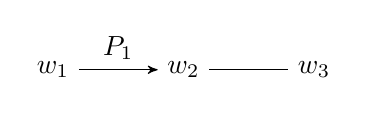
\begin{tikzpicture}[>=stealth']
{[start chain]
\node[on chain] (A) {$w_1$};
\node[on chain,join=by {->,"$P_1$"},right=of A] (B) {$w_2$};
\node[on chain,join=by {-},right=of B] (C) {$w_3$};}
\end{tikzpicture}
\end{center}
\begin{center}
\begin{tabular}{ c|c c c }
& $w_1$ & $w_2$ & $w_3$ \\
\hline 
$h_s(AL(P_1,w_k))$ & $NULL$ & $NULL$ & $NULL$ \\ 
$h_{sf}(AL(P_1,w_k))$ & $NULL$ & $NULL$ & $NULL$ \\ 
Neighbor & $w_2$ & $w_1$ \& $w_3$ & $w_2$\\
\end{tabular}
\end{center}
\end{figure}

\begin{enumerate}
\item $P_1$ sends a signed world entry packet to $w_2$
\item $w_2$ insures that $w_1$ is adjasent to itself
\item $w_2$ must verify that $P_1$ currently resides in $w_1$, this is done by ensuring $h_{sf}(AL(P_1,w_k)) = NULL$. This is found by sending a signed data request to $w_1$ 
\item $P_1$ presents $AL(P_1,w_1)$ to $w_2$
\item $w_1$ calculates $h_s(AL(P_1,w_1))$ using the $AL$ on the serverside
\item $w_2$ calculates $h_s(AL(P_1,w_1))$ using the $AL$ provided by $P_1$, the hashes must match
\item (Optional) An \textbf{Action Ledger Traceback} (\ref{ALT}) can be complete
\item $P_1$ is now granted access to $w_2$ and can submit actions
\item $w_1$ must store $h_s(AL(P_1,w_1))$, $AL(P_1,w_1)$ can be deleted
\end{enumerate}

\begin{figure}
\caption{$P_1$ in $w_2$}
\begin{center}
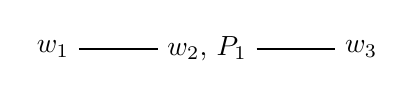
\begin{tikzpicture}[>=stealth']
{[start chain]
\node[on chain] (A) {$w_1$};
\node[on chain,join=by {-},right=of A] (B) {$w_2$, $P_1$};
\node[on chain,join=by {-},right=of B] (C) {$w_3$};}
\end{tikzpicture}
\end{center}
\begin{center}
\begin{tabular}{ c|c c c }
& $w_1$ & $w_2$ & $w_3$ \\
\hline 
$h_s(AL(P_1,w_k))$ & $ h_s(AL(P_1,w_1))$ & $NULL$ & $NULL$ \\ 
$h_{sf}(AL(P_1,w_k))$ & $NULL$ & $NULL$ & $NULL$ \\ 
Neighbor & $w_2$ & $w_1$ \& $w_3$ & $w_2$\\
\end{tabular}
\end{center}
\end{figure}

\begin{figure}
\caption{$P_1$ in $w_3$}
\begin{center}
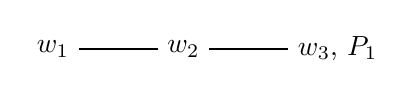
\begin{tikzpicture}[>=stealth']
{[start chain]
\node[on chain] (A) {$w_1$};
\node[on chain,join=by {-},right=of A] (B) {$w_2$};
\node[on chain,join=by {-},right=of B] (C) {$w_3$, $P_1$};}
\end{tikzpicture}
\end{center}
\begin{center}
\begin{tabular}{ c|c c c }
& $w_1$ & $w_2$ & $w_3$ \\
\hline 
$h_s(AL(P_1,w_k))$ & $h_s(AL(P_1,w_1))$ & $h_s(AL(P_1,w_2))$ & $NULL$ \\ 
$h_{sf}(AL(P_1,w_k))$ & $h_s(AL(P_1,w_2))$ & $NULL$ & $NULL$ \\ 
Neighbor & $w_2$ & $w_1$ \& $w_3$ & $w_2$\\
\end{tabular}
\end{center}
\end{figure}

\subsection{Player Genesis} 
\label{PG}
Player Genesis is the creation of a new player, for this to occur a player must digitally sign a genesis package with unix time. The world must ensure there are no existing values entered for that player. The player is then instated into the world with all the initial player values set to zero. 

\subsection{Refuge Package}
\label{RP}
A refugee package is an action ledger that dates to the time that the package is sent. This allows worlds to reinstate players without the need of a world transfer. This is useful for player that have been orphaned into a world. This typically happens during either a \textbf{world disconnect} (\ref{WD}) or \textbf{world outage} (\ref{WO}). This has the effect of splitting the player's history into two forks, which opens the possibility of an \textbf{action ledger conflicts} (\ref{ALC}).

\section{Experience}
\label{exp}
Experience is distributed to players using experience packages. This is simply a package that is of the form shown by figure \ref{exppkg}. When a player is to received experiance this package is hashed, signed and sent to a player from the world. Players are expected to keep all these packages. This same technique can be used to distribute anything to players that doesn't required transferability or fungability. 

\begin{figure}[H]
\centering
\label{exppkg}
\caption{Experience Package}
\begin{lstlisting}
ExpPkg{
	PlayerPublicKey
	WorldPublicKey
	ExpAmount
	ExpType
	UnixTime
}
\end{lstlisting}
\end{figure}

\section{Items} 
% Outstanding issues
% - Player Deaths. What happens to player items?
% - Transferring items to other players. 

\label{items}
Items can be introduced by any node on the network. To spawn an item the item package, defined as $i$, must be signed by the node and submitted to the \textit{worlds smart contract} to prove ownership and lock the funds associated with the item. It is the worlds responsibility to judge which items are credible. This can be done by examining the \textit{WorldPublic} field in the item package, if it has been issued by an adjacent or trusted world the item can be considered real. It is also possible that some worlds might not care if players create items for themselves, in this case the \textit{WorldPublic} would match the \textit{PlayerPublic} field. These options are left completely up to the world creator.

\begin{figure}[H]
\centering
\label{itempkg}
\caption{Item Package $i$ - Wood}
\begin{lstlisting}
ItemName = 'Wood'
ItemClass = 'Material'
ItemHash = hash(ItemName | ItemClass);
PlayerPublic = 0x5d7ac22131ad370e59fddb5f6079a354dbdd2dd9
WorldPublic = 0xb1abdaf3ab936c99f5fd518122cf7d5b811a1a30
Stake = 1WOR
\end{lstlisting}
\end{figure}

\subsection{Worlds Smart Contact}
The worlds smart contract is a contract that keeps track of player possessions. For a player to own an item, the player must possess the item package and for the hash of the item to live on the worlds smart contract. 

\subsection{Item Transfers}
For a player to transfer an item to another player, the player must call the TxItem(ItemHash, PlayerPublic) function.

\subsection{Staked Amounts}
In order for the game theoretical elements of the universe to balance, in order to create an item you must stake some WOR to the item.

\subsection{Forging}
It is possible to forge items by combining multiple items, thus forming a derivative item. In literal sense the act of forging it to call the function \textit{ForgeItem(Item1, Item2, ...)} on the WSC. This will then make a derivative item which is shown in Figure \ref{ForgedItem}. It is up to the worlds to decide on the item names and item classes of these subitems. To forge a sword a player could forge metal, fabric and a sharpening stone. As long at the world recognizes that the resulting hash of these items do in fact form a sword, then the player has crafted a sword for use in these worlds. The power of the sword would be proportional to the amount of stakes WOR in all the items that were used to craft the sword. Once items are forged into something they can no longer be used for anything else. It is possible to unforge an item.

\begin{figure}[H]
\centering
\caption{Forged Item $i_f$}
\label{ForgedItem}
\begin{lstlisting}[escapeinside={(*}{*)}]
ItemHash = hash((*$ParentItemHash_0 | ... | ParentItemHash_n$*))
PlayerPublic = 0x5d7ac22131ad370e59fddb5f6079a354dbdd2dd9
Stake = sum(ParentItemStake)
\end{lstlisting}
\end{figure}

\subsection{Equipping Items}
Depending on the requirement of the world, players may be required to stake items in order to use them. This is a special state where the items enters transient ownership between the player and the world. The world is required to send a signed "pulse" for the player to the WSC to indicate that the player is still alive. If the player is to die, the items will fall under ownership of the world. The world then has the choice to do anything with the items, such as distribute them around the players body for other to collect, return them to the dead player or keep the items as payment for playing in the world. It is wise for world to be transparent as to what happens to player items after the event of a death.

\subsection{Using items}
If a player wants to use an item, it must be transferred to the world the player is currently residing in. 

\section{Currency (WOR)}
\label{money}
A common currency between worlds will be used for staking and integration into the platform. To prevent abuse this currency must be zero sum, meaning worlds cannot generate it and it must start with a fixes supply. Ideally it is tracked through an existing blockchain. Worlds can introduce mechanics for generating revenue, like entrance fees, subscriptions or purchasing items.

\section{Engine Mechanics} 
The mechanics below are simply suggestions. As the engine is completely open, worlds are free to impose whatever mechanics they wish. Worlds with drastically different game mechanics will probably not be bordering, this limits gameplay but maintains fairness. Players are able to play in whatever worlds they wish - but they must start from scratch in non-adjacent clusters.

% Clusters of worlds might be complete anarchy, others built on peace and justice. There will probably not be a connection between sections like this, which is perfectly fine.

\section{System Architecture}
\begin{center}
\begin{tabular}{r l}
$A$: & Action\\ 
$Cy(A)$: & Signed Action\\
$R$: & Response\\ 
$Cy(R)$: & Signed Response\\

\end{tabular}
\end{center}

\begin{small}
\tikzset{myblock/.style = {rectangle, draw, minimum height=1cm, minimum width=3cm}}
\begin{center}
\begin{tikzpicture}
\node(WE)[myblock]{\begin{tabular}{c}Worlds Engine \\ {\scriptsize wClient.py} \\\end{tabular}};
\node (WS)[myblock,above of=WE, yshift=1cm]{\begin{tabular}{c}Worlds Server \\ {\scriptsize wServer.py} \\\end{tabular}};
\node (WC)[myblock,left of=WE, xshift=-3cm]{\begin{tabular}{c}Game Client \\ {\scriptsize \textit{From game Dev}} \\\end{tabular}};
\node (Key)[myblock,below of=WE, yshift=-1cm]{\begin{tabular}{c}Key Pair \\ {\scriptsize private.pem/public.pem} \\\end{tabular}};
\node (AL)[myblock,right of=Key, xshift=3cm]{\begin{tabular}{c}Action Ledger \\ {\scriptsize AL/} \\\end{tabular}};
\node (AList)[myblock,left of=Key, xshift=-3cm]{\begin{tabular}{c}Action Listing \\ {\scriptsize ActionListing.yaml} \\\end{tabular}};
\node (PF)[myblock,below of=AList, yshift=-1cm]{\begin{tabular}{c}Player File \\ {\scriptsize player.yaml} \\\end{tabular}};

\draw[->] ($(WE.north east)!0.25!(WE.north west)$) -- node[anchor=west]{$Cy(A)$} ($(WS.south east)!0.25!(WS.south west)$);
\draw[<-] ($(WE.north east)!0.75!(WE.north west)$) -- node[anchor=west]{$Cy(R)$} ($(WS.south east)!0.75!(WS.south west)$);
\draw[->] (WC) -- node[anchor=north]{$A$} (WE);
\draw[<-] (WE) -- (Key);
\draw[<->] (AList) -- (WC);
\draw ($(AList.north east)!0.25!(AList.north west)$)edge[out=90,in=-90,->]($(WE.south east)!0.75!(WE.south west)$);
\draw ($(AL.north east)!0.5!(AL.north west)$)edge[out=90,in=-90,<->]($(WE.south east)!0.25!(WE.south west)$);
\draw ($(PF.north)!0.5!(PF.north)$)edge[out=90,in=-90,<-]($(WE.south east)!0.63!(WE.south west)$);
\draw ($(PF.north west)!0.5!(PF.south west)$)edge[out=180,in=-180,->]($(WC.south west)!0.5!(WC.north west)$);

% more arrows here
\end{tikzpicture}
\end{center}
\end{small}

\section{Outstanding Issues}

\subsection{Malicious Worlds}

\end{document}
